%%%%%%%%%%%%%%%%%%%%%%%%%%%%%%%%%%%%%%%%%
% Beamer Presentation
% LaTeX Template
% Version 1.0 (10/11/12)
%
% This template has been downloaded from:
% http://www.LaTeXTemplates.com
%
% License:
% CC BY-NC-SA 3.0 (http://creativecommons.org/licenses/by-nc-sa/3.0/)
%
%%%%%%%%%%%%%%%%%%%%%%%%%%%%%%%%%%%%%%%%%

%----------------------------------------------------------------------------------------
%	PACKAGES AND THEMES
%----------------------------------------------------------------------------------------

\documentclass{beamer}

\mode<presentation> {

% The Beamer class comes with a number of default slide themes
% which change the colors and layouts of slides. Below this is a list
% of all the themes, uncomment each in turn to see what they look like.

%\usetheme{default}
%\usetheme{AnnArbor}
%\usetheme{Antibes}
%\usetheme{Bergen}
%\usetheme{Berkeley}
%\usetheme{Berlin}
%\usetheme{Boadilla}
%\usetheme{CambridgeUS}
%\usetheme{Copenhagen}
%\usetheme{Darmstadt}
%\usetheme{Dresden}
%\usetheme{Frankfurt}
%\usetheme{Goettingen}
%\usetheme{Hannover}
%\usetheme{Ilmenau}
%\usetheme{JuanLesPins}
%\usetheme{Luebeck}
\usetheme{Madrid}
%\usetheme{Malmoe}
%\usetheme{Marburg}
%\usetheme{Montpellier}
%\usetheme{PaloAlto}
%\usetheme{Pittsburgh}
%\usetheme{Rochester}
%\usetheme{Singapore}
%\usetheme{Szeged}
%\usetheme{Warsaw}

% As well as themes, the Beamer class has a number of color themes
% for any slide theme. Uncomment each of these in turn to see how it
% changes the colors of your current slide theme.

%\usecolortheme{albatross}
%\usecolortheme{beaver}
%\usecolortheme{beetle}
%\usecolortheme{crane}
%\usecolortheme{dolphin}
%\usecolortheme{dove}
%\usecolortheme{fly}
%\usecolortheme{lily}
%\usecolortheme{orchid}
%\usecolortheme{rose}
%\usecolortheme{seagull}
%\usecolortheme{seahorse}
%\usecolortheme{whale}
%\usecolortheme{wolverine}

%\setbeamertemplate{footline} % To remove the footer line in all slides uncomment this line
%\setbeamertemplate{footline}[page number] % To replace the footer line in all slides with a simple slide count uncomment this line

%\setbeamertemplate{navigation symbols}{} % To remove the navigation symbols from the bottom of all slides uncomment this line
}

\usepackage{graphicx} % Allows including images
\usepackage{booktabs} % Allows the use of \toprule, \midrule and \bottomrule in tables
\usepackage{multirow}
\usepackage{adjustbox}
\usepackage{array}
\usepackage{tikz}
\usetikzlibrary{shapes.geometric, arrows, positioning, fit}
\usepackage[latin1]{inputenc}
\newcommand{\xmark}{\textcolor{red}{\text{\sffamily X}}}
\newcommand{\cmark}{\textcolor{green}{\checkmark}}
\newcommand{\tr}{\text{tr}}
\newcommand{\E}{\textbf{E}}
\newcommand{\diag}{\text{diag}}
\newcommand{\argmax}{\text{argmax}}
\newcommand{\argmin}{\text{argmin}}
\newcommand{\Cov}{\text{Cov}}
\newcommand{\Var}{\text{Var}}
\newcommand{\Vol}{\text{Vol}}
\newcommand{\bx}{\boldsymbol{x}}
\newcommand{\by}{\boldsymbol{y}}
\newcommand{\bX}{\boldsymbol{X}}
\newcommand{\bY}{\boldsymbol{Y}}

%tikz stufff


%----------------------------------------------------------------------------------------
%	TITLE PAGE
%----------------------------------------------------------------------------------------


\title[Informal]{How many neurons does it take to classify a lightbulb?}

\author{Charles Zheng} % Your name
\institute[Stanford] % Your institution as it will appear on the bottom of every slide, may be shorthand to save space
{Stanford University}
\date{\today} % Date, can be changed to a custom date

\begin{document}

\begin{frame}
\titlepage % Print the title page as the first slide
(Joint work with Yuval Benjamini.)
\end{frame}

\begin{frame}
\frametitle{Overview}
\noindent\emph{Introduction}
\begin{itemize}
\item Review of information theory.
\item Study of neural coding.
\end{itemize}
\noindent\emph{Related work}
\begin{itemize}
\item Estimating mutual information between stimulus and response.
\item Can we use machine learning methods to estimate MI?
\end{itemize}
\noindent\emph{Theory}
\begin{itemize}
\item Gaussian example.
\item Low-SNR universality.
\end{itemize}
\noindent\emph{Results}
\end{frame}

\section{Introduction}

\begin{frame}
\frametitle{Information theory} 
The high performance and reliability of modern communications system is made possible by information theory, founded by Shannon in 1948.
\vspace{0.4in}
\begin{center}
\begin{tabular}{cc}
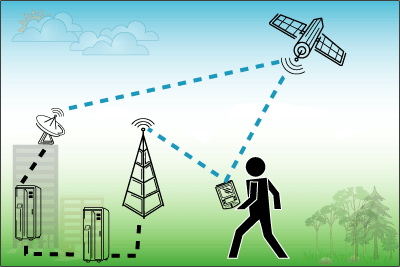
\includegraphics[scale =0.3]{communication-entry.png} &
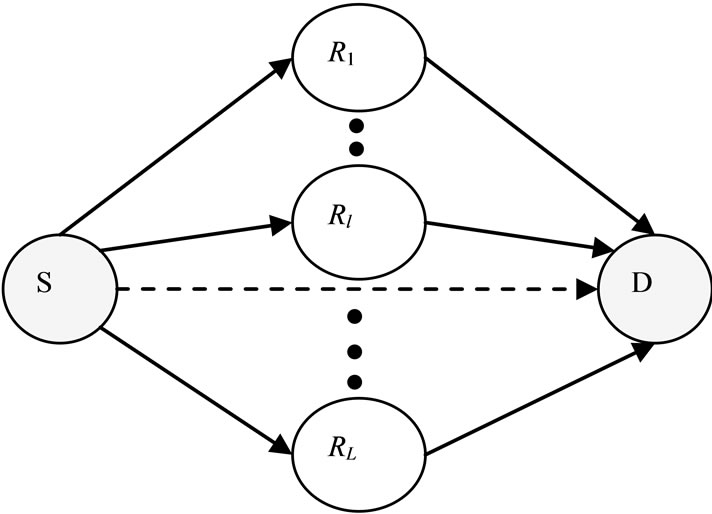
\includegraphics[scale =  0.2]{relay_channel.jpg}
\end{tabular}
\end{center}
\vspace{0.4in}
A information-processing network can be analyzed in terms of interactions between its components (which are viewed as random variables.)

\tiny{Image credit CartouCHe, Aziz et al. 2011.}
\note{ Modern communication systems depend
  on a vast network of signal transmitters and receivers.  All of this
  sophisticated engineering is made possible by information theory, a
  branch of applied mathematics introduced by Claude Shannon in 1948.
  Under the lens of information theory, we decompose a information
  network (e.g. the internet) into individual components (e.g. a
  server, a satellite) and view this collection of components as a
  collection of random variables, similar to a probabilistic graphical
  model.  Information theory defines quantities such as entropy,
  conditional entropy, and mutual information which serve to quantify
  how much information is contained in each component, and how the
  information is transmitted or lost as it passes through the network.
}
\end{frame}

\begin{frame}
\frametitle{Entropy and mutual information}
$X$ and $Y$ have joint density $p(x, y)$ with respect to $\mu$.

\vspace{0.5in}

\begin{tabular}{c|c|c}
\hline
Quantity & Definition & Linear analogue\\\hline
Entropy & $H(X) = - \int (\log p(x)) p(x) \mu_X(dx)$ & $\text{Var}(X)$\\
Conditional entropy & $H(X|Y) = \E[H(X|Y)]$ & $\E[\text{Var}(X|Y)]$\\
Mutual information & $I(X;Y) = H(X) - H(X|Y)$ & $\text{Cor}^2(X, Y)$\\\hline
\end{tabular}

\vspace{0.3in}

\small{The above definition includes both \emph{differential} entropy and \emph{discrete} entropy.
Information theorists tend to use log base 2, we will use natural logs in this talk.}
\end{frame}

\begin{frame}
\frametitle{Properties of mutual information}
\begin{center}
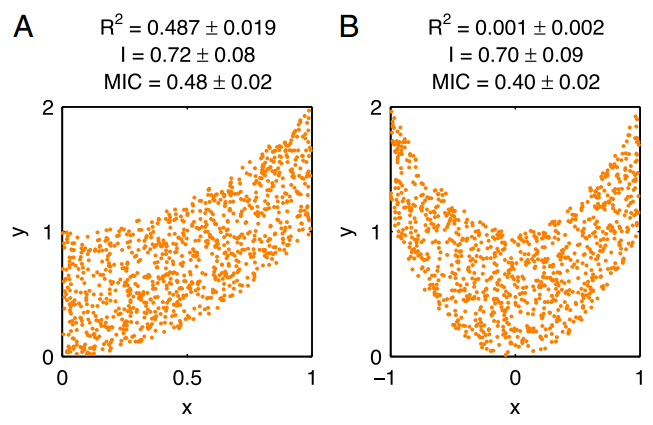
\includegraphics[scale = 0.2]{kinney.png}
\end{center}
\begin{itemize}
\item $I(X;Y) \in [0,\infty]$.  (0 if $X \perp Y$, $\infty$ if $X=Y$ and $X$ continuous.)
\item Symmetry: $I(X;Y) = I(Y; X)$.
\item Data-processing inequality
\[I(X; Y) \geq I(\phi(X); \psi(Y))\]
equality for $\phi$, $\psi$ bijections
\item Additivity.  If $(X_1,Y_1) \perp (X_2, Y_2)$, then
\[
I((X_1, X_2); (Y_1, Y2)) = I(X_1; Y_1) + I(X_2; Y_2).
\]
%\item Relation to KL divergence
%\[\mathbb{D}(p(x, y)||p(x)p(y)) = I(X; Y).\]
\end{itemize}
\tiny{Image credit Kinney et al. 2014.}
\end{frame}

\begin{frame}
\frametitle{Relationship between mutual information and classification}
\begin{itemize}
\item Suppose $X$ and $Y$ are discrete random variables, and $X$ is uniformly distributed over its support.
\item Classify $X$ given $Y$.  The optimal rule is to guess
\[
\hat{X} = \argmax_x\ p(Y|X=x).
\]
\item Bayes error:
\[
p_e = \Pr[X \neq \hat{X}].
\]
\item Fano's inequality:
\[
I(X; Y) \geq (1-p_e) \ln K - \text{const.}
\]
where $K$ is the size of the support of $X$.
\end{itemize}
\end{frame}

\begin{frame}
\frametitle{Nice interpretation of $I(X; Y)$ for continuous rvs}
\begin{itemize}
\item If we bin the continuous $X$ into $K \approx e^{I(X; Y)}$ equal-probability bins,
we can reliably guess the bin given $Y$.
\item Heuristic is more accurate if $I(X; Y)$ is large, due to Shannon's noisy channel theorem.
\end{itemize}
\begin{center}
\begin{tabular}{ccc}
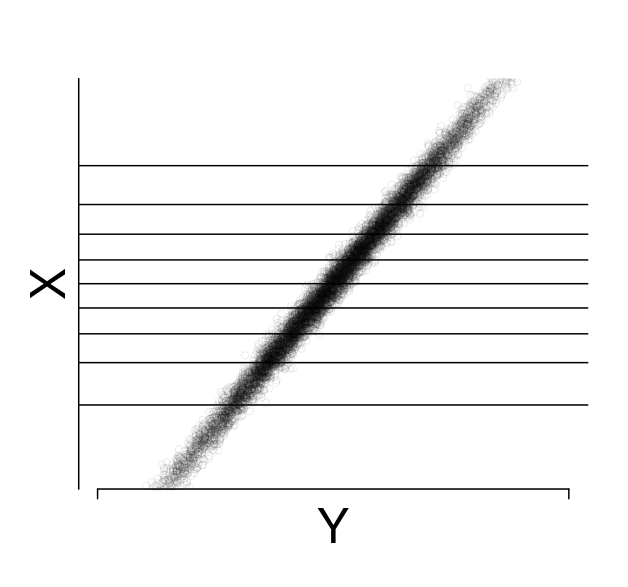
\includegraphics[scale = 0.23]{../info_theory_paper/bin_figure1.png} & &
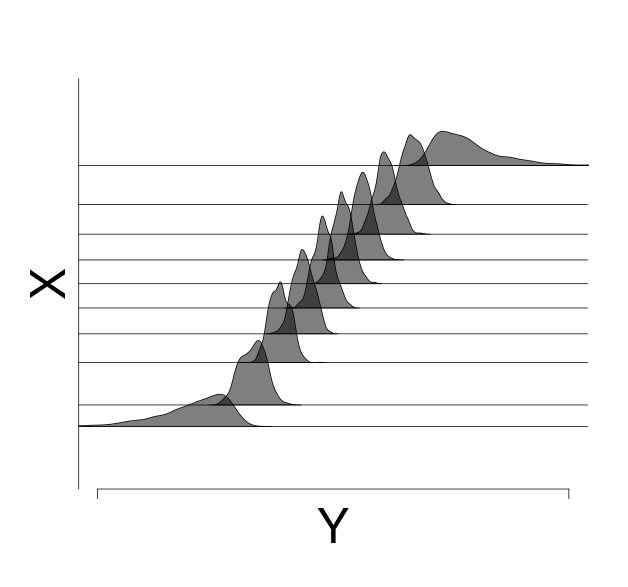
\includegraphics[scale = 0.23]{../info_theory_paper/bin_figure1a.png}\\
$I(X; Y) = 2.3038$ & & $\ln 10 = 2.3025$
\end{tabular}
\end{center}
\note{This is another way of seeing that $I(X;Y)$ is bijection invariant.}
\end{frame}

\begin{frame}
\frametitle{Motivation: the neural code}
The brain is the \emph{most complex} information processing system we know!
\vspace{0.3in}
\begin{center}
\begin{tabular}{cc}
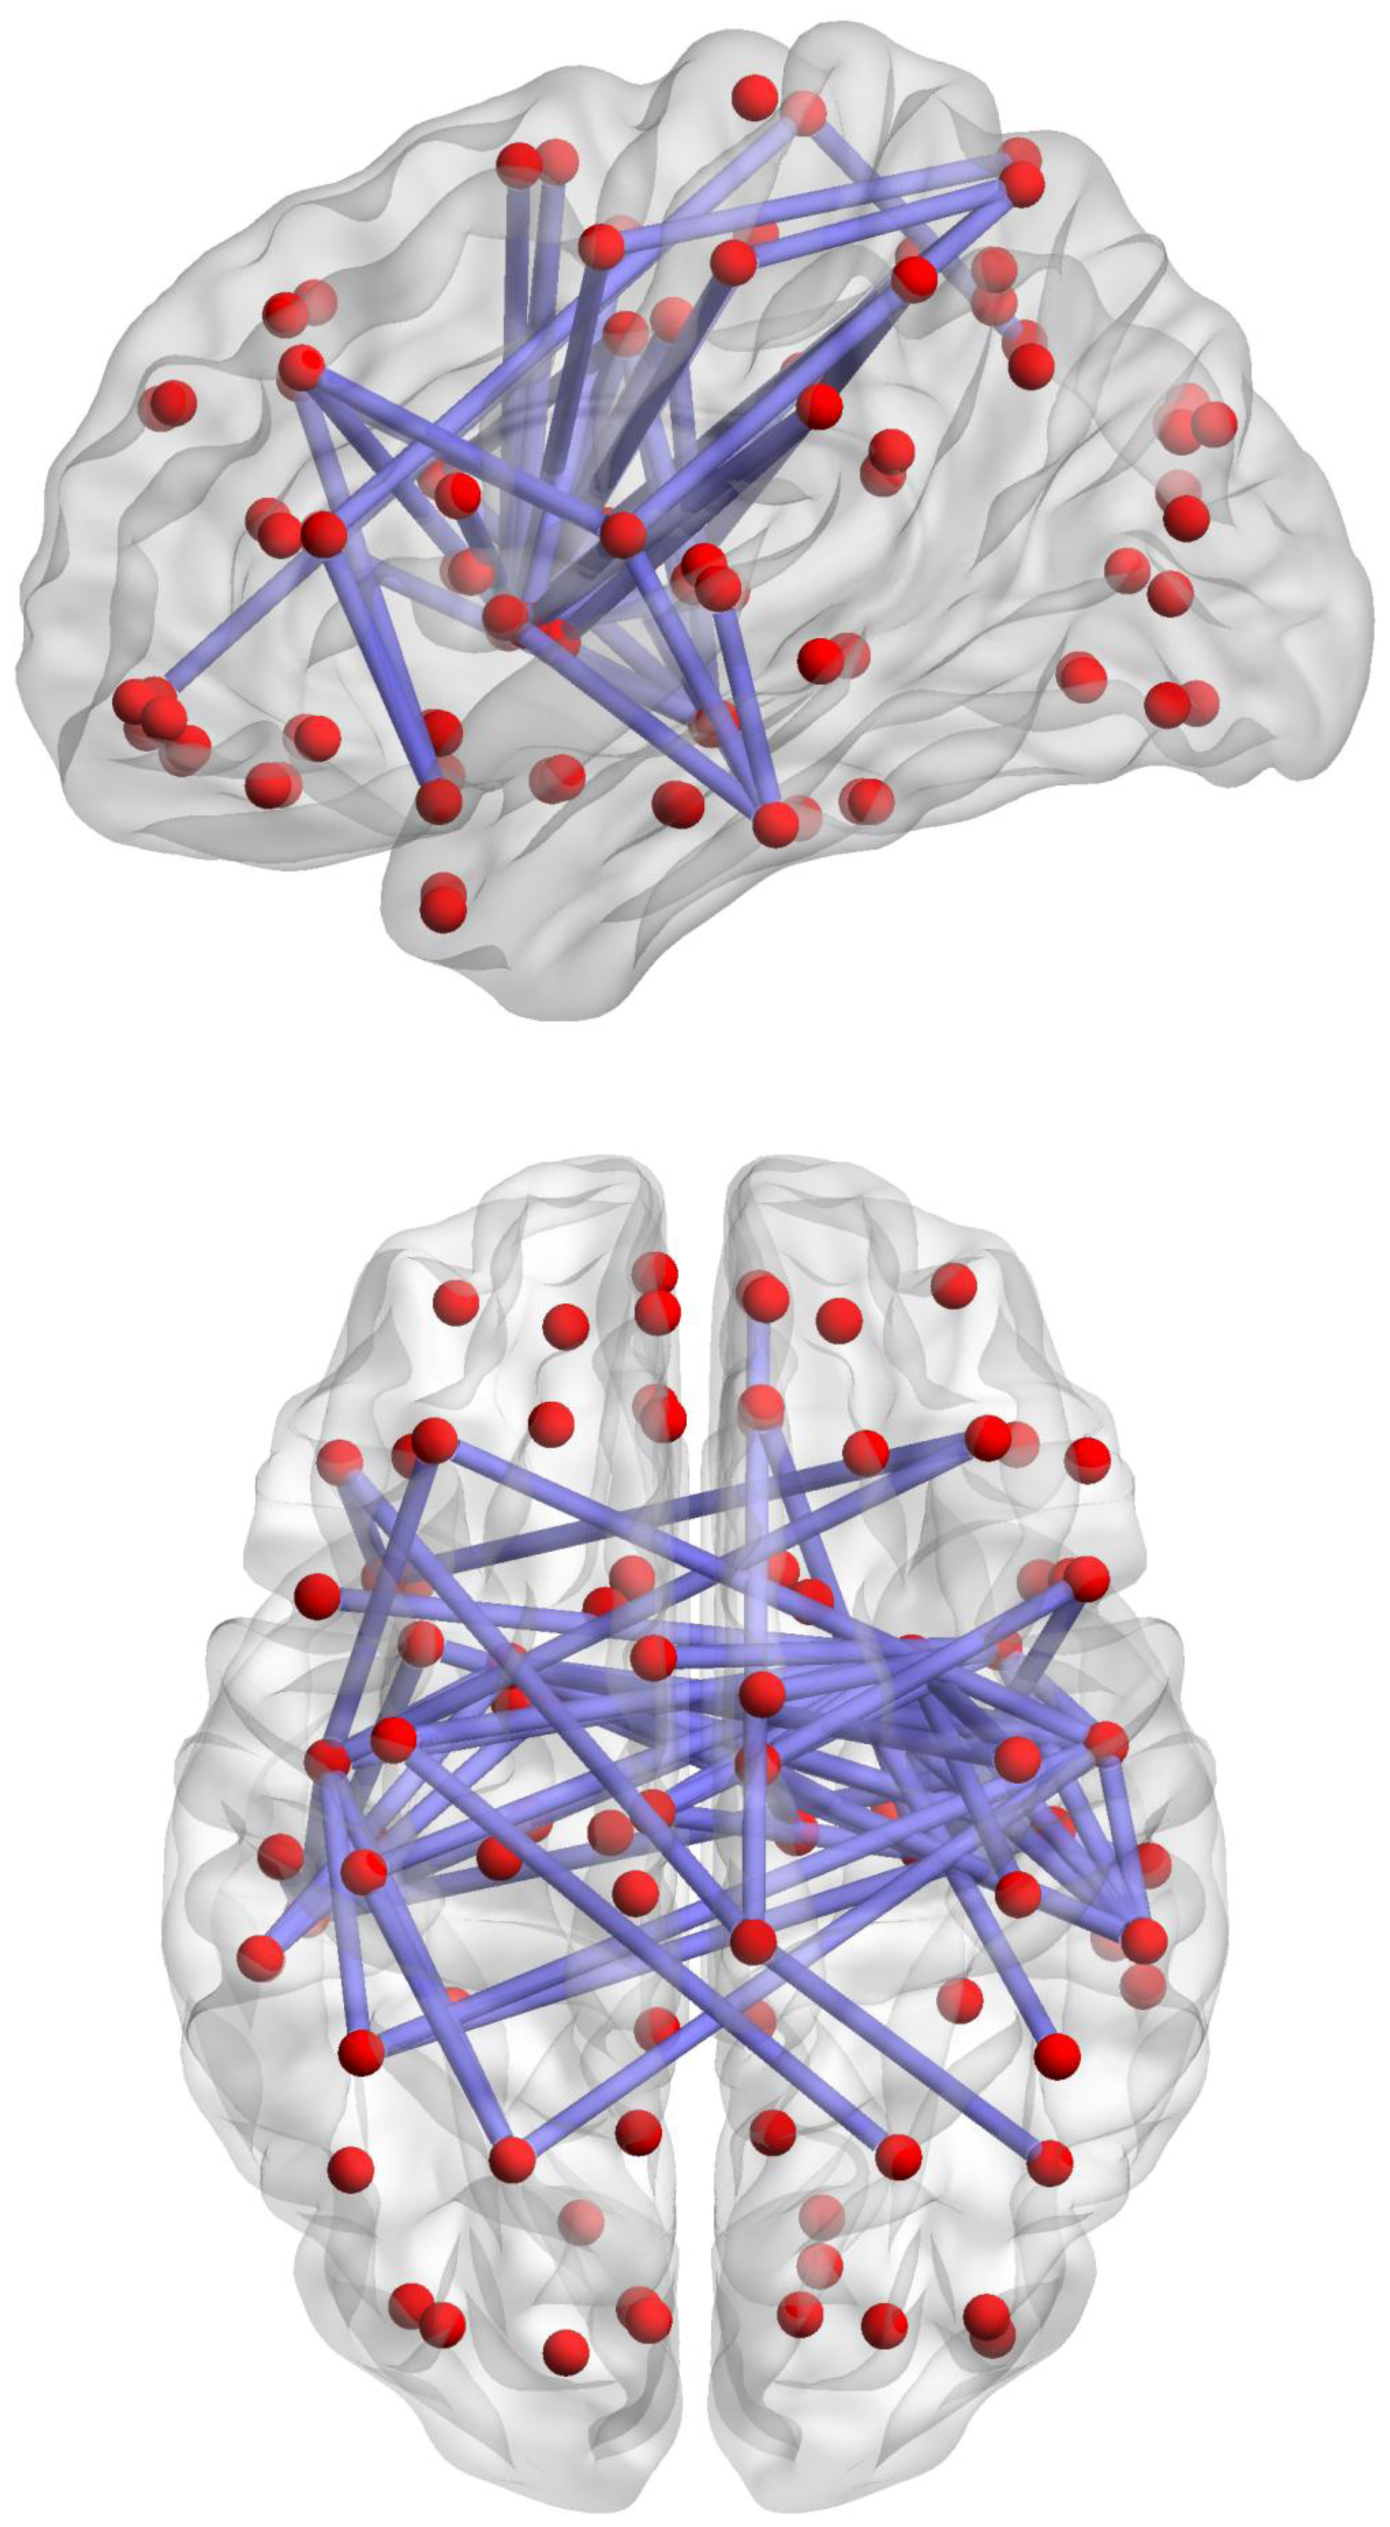
\includegraphics[scale = 0.3, clip =true, trim=0 0 0 2.5in]{Brain_network.png} &
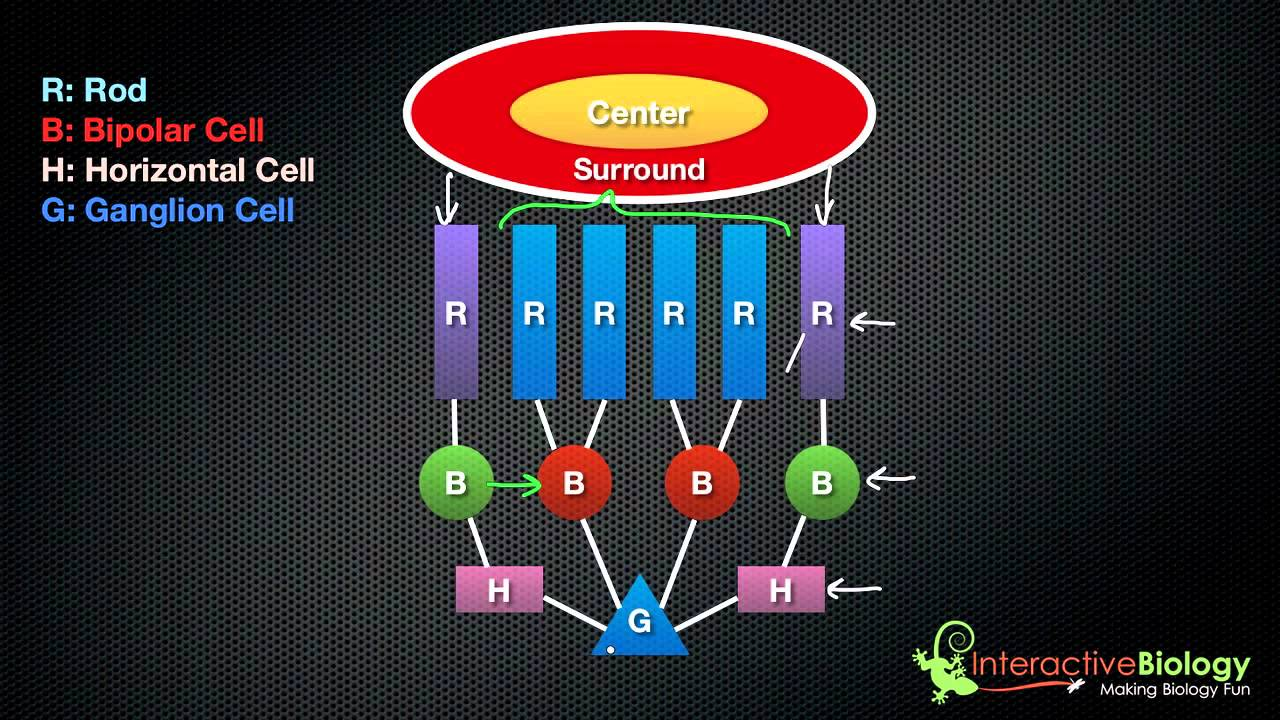
\includegraphics[scale = 0.1]{maxresdefault.jpg}\\
\small{Neural network inferred from data.} & \small{Organization of human retina}\\
\small{(Hong et al.)} & 
\end{tabular}
\end{center}
\vspace{0.3in}
How do neurons encode, process, and decode sensory information?

\tiny{Image credit: Hong et al., Interactive Biology}
\end{frame}


\begin{frame}
\frametitle{Studying the neural code: data}
\begin{center}
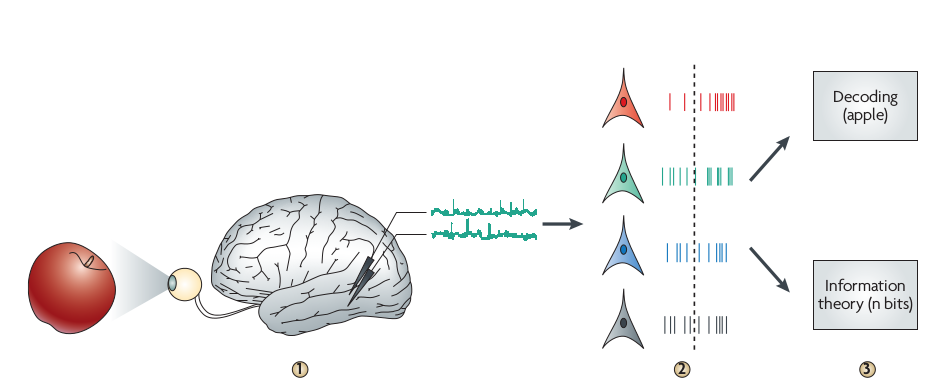
\includegraphics[scale = 0.2]{quiroga.png}
\end{center}
\begin{itemize}
\item  Let $\mathcal{X}$ define a class of stimuli (faces, objects, sounds.)
\item Stimulus $\bX = (X_1,\hdots, X_p)$, where $X_i$ are features (e.g. pixels.)
\item Present $\bX$ to the subject, record the subject's brain activity using EEG, MEG, fMRI, or calcium imaging.
\item Recorded response $\bY = (Y_1,\hdots, Y_q)$, where $Y_i$ are single-cell responses, or recorded activities in different brain region. 
\end{itemize}
\tiny{Image credits: Quiroga et al. (2009).}
\end{frame}




\begin{frame}
\frametitle{Problem statement}
Given stimulus-reponse data $(\bX, \bY)$, can we estimate the mutual information $I(\bX; \bY)$?

\vspace{0.5in}
\emph{Why do we care?}
\begin{itemize}
\item Assessing quality of \emph{pre-processing.}
\item Selecting the correct model for neural encoding.
\item Assessing the \emph{efficiency} of the neural code.
\item Measuring the \emph{redundancy} of a population of neurons
\[
r' = \frac{\sum_{i=1}^q I(\bX; Y_i) - I(\bX; \bY)}{\sum_{i=1}^q I(\bX; Y_i)}.
\]
\end{itemize}
\end{frame}


\begin{frame}
\frametitle{Experimental design}
\begin{itemize}
\item How to make inferences about the population of stimuli in
  $\mathcal{X}$ using finitely many examples?
\item \emph{Randomization.}  Select $\bX^{(1)},\hdots,
  \bX^{(K)}$ randomly from some distribution $p(\bx)$ (e.g. an image
  database).  Record $r$ responses from each stimulus.
\end{itemize}
\begin{center}
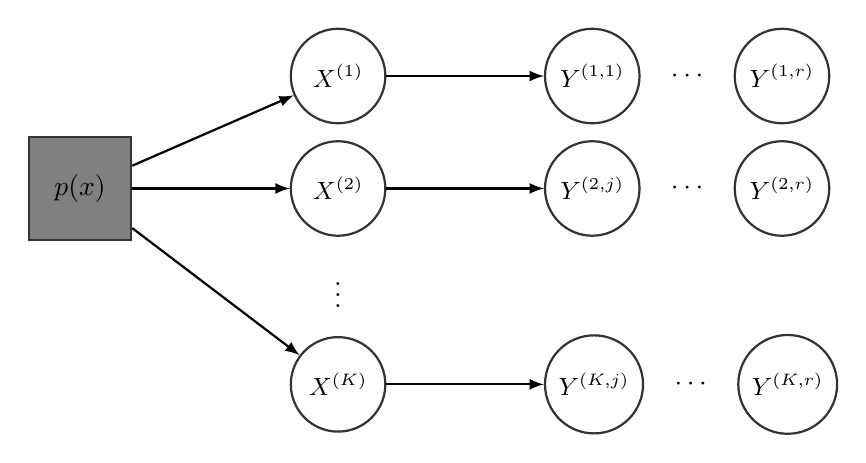
\begin{tikzpicture}[node distance = 2mm and 20mm]
\tikzstyle{main} = [circle, minimum size = 12mm, thick, draw = black!80]
\tikzstyle{main0} = [circle, minimum size = 2mm, thick, draw = white!100]
\tikzstyle{param} = [rectangle, minimum size = 13mm, thick, draw = black!80]
\tikzstyle{connect} = [-latex, thick]
\tikzstyle{box} = [rectangle, draw = black!100]
  \node[param, fill = black!50] (px) {$p(\bx)$};
  \node[main, right=of px] (x2) {\small{$\bX^{(2)}$}};
  \node[main, above=of x2] (x1) {\small{$\bX^{(1)}$}};
  \node[main0, below=of x2] (xdots) {$\vdots$};
  \node[main, below=of xdots] (x3) {\small{$\bX^{(K)}$}};
  \node[main, right=of x1] (y11) {\small{$\bY^{(1,1)}$}};
  \node[main, right=of x2] (y21) {\small{$\bY^{(2,j)}$}};
  \node[main, right=of x3] (y31) {\small{$\bY^{(K,j)}$}};
\begin{scope}[node distance = 3mm and 2mm]
  \node[main0, right=of y11] (y12) {$\cdots$};
  \node[main0, right=of y21] (y22) {$\cdots$};
  \node[main0, right=of y31] (y32) {$\cdots$};
  \node[main, right=of y12] (y13) {\small{$\bY^{(1,r)}$}};
  \node[main, right=of y22] (y23) {\small{$\bY^{(2,r)}$}};
  \node[main, right=of y32] (y33) {\small{$\bY^{(K,r)}$}};
\end{scope}
\path (px) edge [connect] (x1) (px) edge [connect] (x2) (px) edge [connect] (x3)
      (x1) edge [connect] (y11) (x2) edge [connect] (y21) (x3) edge [connect] (y31);
\end{tikzpicture}
\end{center}
\end{frame}

\section{Related work}

\begin{frame}
\frametitle{Can we learn $I(\bX; \bY)$ from such data?}
Answer: yes.
\begin{itemize}
\item We have $I(\bX; \bY) = H(\bY) - H(\bY|\bX)$.
\item We can estimate $H(\bY)$ from the data
\item We can estimate $H(\bY| \bx^{(i)})$ from the data, and define
\[
\hat{H}(\bY|\bX) = \frac{1}{K}\sum_{i=1}^K \hat{H}(\bY| \bX^{(i)})
\]
\item As $K$ and $r$ both tend to infinity, 
\[
\hat{I}(\bX; \bY) = \hat{H}(\bY) - \hat{H}(\bY|\bX)
\]
is consistent for $I(\bX; \bY)$.
\end{itemize}
\end{frame}

\begin{frame}
\frametitle{Limitations with the `na\"{i}ve' approach}
Na\"{i}ve estimator:
\[
\hat{I}(\bX; \bY) = \hat{H}(\bY) - \frac{1}{K}\sum_{i=1}^K \hat{H}(\bY| \bX^{(i)})
\]
\begin{itemize}
\item If $K$ is small, the na\"{i}ve estimator may be quite biased, even for low-dimensional problems.
Gastpar et al. (2010) introduced an \emph{antropic correction} to deal with the small-$K$ bias.
\item Difficult to estimate differential entropies $H(\bY),\
  H(\bY|\bx^{(i)})$ in high dimensions.  Best rates are
  $O(1/\sqrt{n})$ for $d \leq 3$ dimensions.  Convergence rates for $d > 3$
  unknown!
\end{itemize}
\end{frame}

\begin{frame}
\frametitle{Can we use machine learning to deal with dimensionality?}
\begin{itemize}
\item Supervised learning becomes an extremely common approach for dealing with high-dimensional data, for numerous reasons!
\item Perhaps we can use supervised learning to estimate $I(\bX; \bY)$ as well.
\end{itemize}
\emph{Procedure.}
\begin{itemize}
\item Fix $r_{train} < r$.  Let $r_{test} = r - r_{train}$.
\item Use $\{(\bx^{(i)}, \by^{(i, j)}): i = 1,\hdots, K, j = 1,\hdots, r_{train}\}$ as training data to learn a classifier $\hat{\bx}$.
\item Compute the confusion matrix, normalized so that each row adds to $1/K$:
\[
C(i, j) = \frac{1}{K^2 r_{test}} \sum_{i=1}^K \sum_{j=1}^K  \sum_{\ell=r_{train} + 1}^r I(\hat{\bx}(\by^{(i,\ell)}) = \bx^{(j)}).
\]
\end{itemize}
Normalized this way, $C(i, j)$ gives the empirical joint distribution
\[
C(i, j) = \hat{\Pr}[\bX = \bx^{(i)}, \hat{\bX} = \bx^{(j)}].
\]
\end{frame}

\begin{frame}
\frametitle{Can we use machine learning to deal with dimensionality?}
\begin{itemize}
\item Treves et al. (1997) suggest computing the mutual information from the confusion matrix,
i.e.
\[
\hat{I}(\bX; \bY) \approx 
\sum_{i=1}^K \sum_{j = 1}^K 
C(i, j) \ln\left(\frac{C(i, j)}{\left(\sum_{\ell=1}^K C(i, \ell)\right) \left(\sum_{\ell=1}^k C(\ell, j) \right)}\right)
\]
\item Quiroga (2009) review the applications of this approach, and note sources of bias or ``information loss.''
\end{itemize}
\end{frame}

\begin{frame}
\frametitle{Why use supervised learning to estimate $I(\bX; \bY)$?}

\begin{itemize}
\item Successful supervised learning exploits structure in the data, which \emph{nonparametric methods ignore.}
\item Using supervised learning to estimate mutual information can be viewed as \emph{using prior information} to improve the estimate of $I(\bX; \bY)$.
\item So while the general problem of information estimation is nearly impossible in high dimensions,
the problem might become tractable if we can exploit known structure in the problem!
\end{itemize}
\end{frame}

\begin{frame}
\frametitle{Interesting connection to machine learning literature}

While we are considering
\[
\text{supervised learning} \to \text{estimate mutual information},
\]
a vast literature exists on applications of mutual information (as the `infomax criterion`) for feature selection, training objectives, i.e.
\[
\text{estimate mutual information} \to \text{supervised learning}.
\]
\end{frame}

\section{Methods}

\begin{frame}
\frametitle{Questions}
\begin{itemize}
\item How much could we potentially gain in estimating $I(\bX; \bY)$ by using supervised learning, compared to nonparametric approaches?
\item Is the Bayes confusion matrix sufficient for consistently estimating $I(\bX; \bY)$?
\item Is the Bayes error sufficient for consistently estimating $I(\bX; \bY)$?
\item In practice, we cannot obtain the Bayes error due to:
\begin{itemize}
\item Model mispecification.
\item Finite training data to fit the model (even if correctly specified).
\item Finite test data to estimate the generalization error.
\end{itemize}
How sensitive is our estimator to these issues?
\end{itemize}
\end{frame}

\begin{frame}
\frametitle{Gaussian example}
To help think about these problems, consider a concrete example:
\begin{itemize}
\item Let $\bX \sim N(0, I_d)$ and 
$\bY|\bX \sim N(\bX,\sigma^2 I_d)$.
\item We draw stimuli $\bx^{(1)}, \hdots, \bx^{(K)} \sim N(0, I_d)$ i.i.d.
\item For each stimulus $\bx^{(i)}$, we draw observations $\by^{(i, j)} = \bx^{(i)} + \epsilon^{(i, j)}$, where $\epsilon^{(i, j)} \sim N(0, \sigma^2 I_d)$.
\end{itemize}
\begin{center}
\begin{tabular}{ccc}
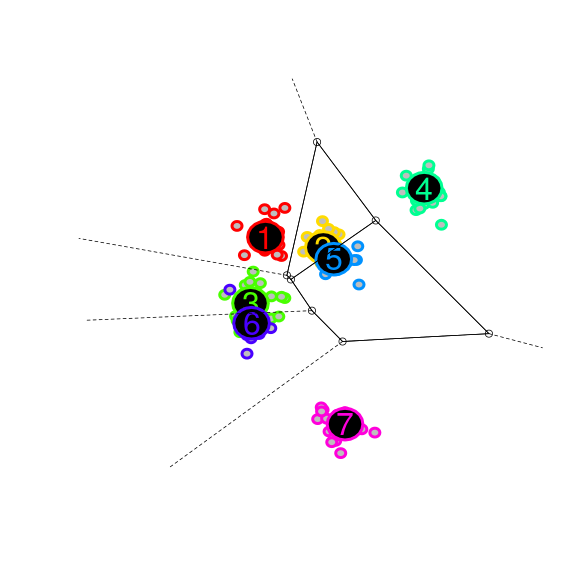
\includegraphics[scale = 0.2, clip = true, trim = 0.6in 0.2in 0.6in 0.2in]{../info_theory_paper/gaussian_figure1a.png} &
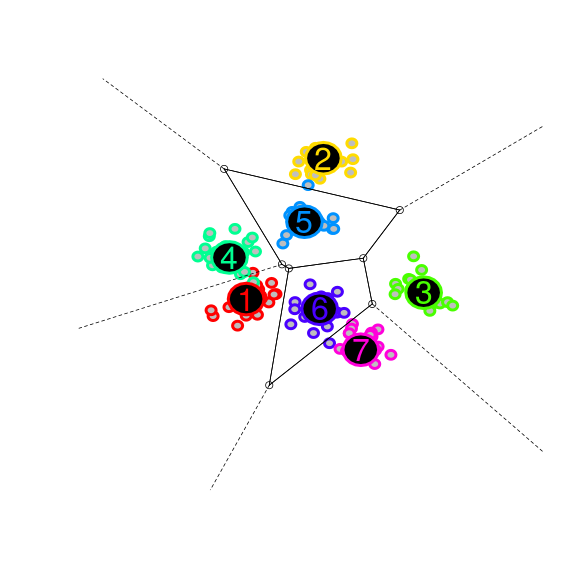
\includegraphics[scale = 0.2, clip = true, trim = 0.6in 0.2in 0.6in 0.2in]{../info_theory_paper/gaussian_figure1b.png} &
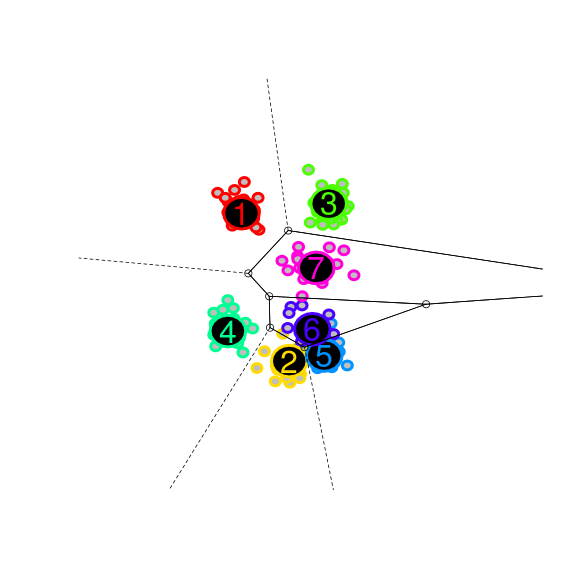
\includegraphics[scale = 0.2, clip = true, trim = 0.6in 0.2in 0.6in 0.2in]{../info_theory_paper/gaussian_figure1c.png}
\end{tabular}
\end{center}
\end{frame}

\begin{frame}
\frametitle{Gaussian example}
The mutual information is given by
\[
I(\bX;\bY) = \frac{d}{2}\log(1 + \frac{1}{\sigma^2}).
\]

The Bayes rule takes the form
\[
\hat{\bX}(\bY) = \argmax_{\bx^{i}} \underbrace{-\frac{1}{2\sigma^2} ||\bY - \bx||^2}_{Z_i}.
\]

\emph{Notation:}
Without loss of generality, assume $\bY$ belongs to the centroid $\bx^{(K)}$.
Then write $\bx^* = \bx^{(K)}$ and $Z_* = Z_K$.

The average Bayes error can be written
\[
\text{ABE} = \Pr[Z_* < \max_{i=1}^{K-1} Z_i].
\]
\end{frame}

\begin{frame}
\frametitle{Gaussian example: Average Bayes error}

\begin{center}
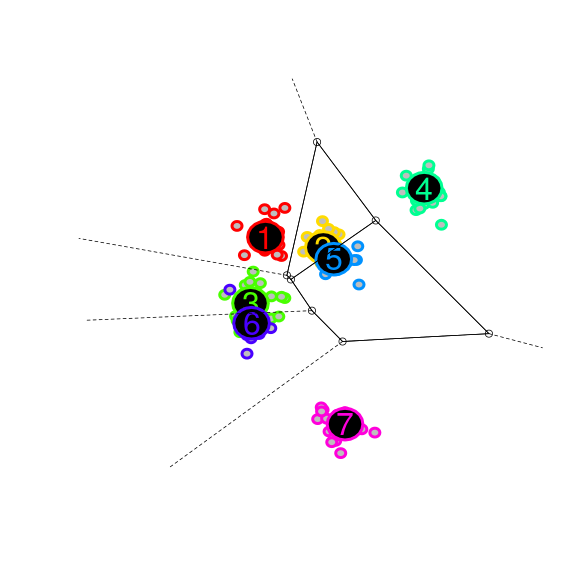
\includegraphics[scale = 0.3, clip = true, trim = 0.6in 3in 0.6in 1.5in]{../info_theory_paper/gaussian_figure1a.png}
\end{center}

\begin{itemize}
\item Conditional on the centroid locations $\bx^{(1)},\hdots,
  \bx^{(K)}$, the Bayes misclassification error can be computed by
  integrating $p$-dimensional Gaussian density over Voronoi polytopes.
\item This is pretty much intractable in high dimensions!
\item The average Bayes error (ABE) is an average of
  an intractable quantity.  Luckily, \emph{taking averages makes
    the problem tractable}.
\end{itemize}
\end{frame}

\begin{frame}
\frametitle{Gaussian example: Average Bayes risk}
\begin{itemize}
\item To make the problem even easier, we use another time-honored technique: the central limit theorem.
\item Letting $d \to \infty$, the scores
\[
Z_i = -\frac{1}{2\sigma^2} ||\bY - \bx||^2 = -\frac{1}{2\sigma^2} \sum_{i=1}^d ||Y_i - x_i||^2
\]
have a jointly multivariate distribution in the limit:
\end{itemize}
\[
\begin{bmatrix}
Z_*\\
Z_1\\
\vdots\\
Z_{K-1}
\end{bmatrix} \stackrel{d}{\to} N\left(
\begin{bmatrix}
-\frac{d}{2}\\
-\frac{d}{2} - \frac{d}{\sigma^2}\\
\vdots\\
-\frac{d}{2} - \frac{d}{\sigma^2}
\end{bmatrix},
\begin{bmatrix}
\frac{d}{2} & \frac{d}{2} & \cdots & \frac{d}{2}\\
\frac{d}{2} & \frac{d}{2} + \frac{2d}{\sigma^2} & \cdots & \frac{d}{2} + \frac{d}{\sigma^2}\\
\vdots & \vdots & \ddots & \vdots\\
\frac{d}{2} & \frac{d}{2} + \frac{d}{\sigma^2} & \cdots & \frac{d}{2} + \frac{2d}{\sigma^2}
\end{bmatrix}
\right).
\]
\end{frame}

\begin{frame}
\frametitle{Gaussian example: Average Bayes risk}

Assume $(Z_*, Z_1,\hdots, Z_{K-1})$ have a normal distribution with the given moments.

We can compute
\[
\text{ABE} = \Pr[Z_* < \max_{i=1}^{K-1} Z_i]
\]
by writing
\[
Z_i = \frac{\Cov(Z_*, Z_i)}{\Var(Z_*)} (Z_* - \E Z_*) + \sqrt{\Var(Z_i) - \frac{\Cov(Z_*, Z_i)^2}{\Var(Z_*)}} W_i,
\]
where $W_i$ are i.i.d. standard normal.

This yields
\[
\Pr[Z_* < \max_{i=1}^{K-1} Z_i] = \Pr[N(\mu, \nu^2) < \max_{i=1}^{K-1} W_i]
\]
where
\[
\mu = \frac{\E[Z_* - Z_i]}{\sqrt{\frac{1}{2}\Var(Z_i - Z_j)}},\ \nu^2 = \frac{\Cov(Z_* - Z_i, Z_* - Z_j)}{\frac{1}{2}\Var(Z_i - Z_j)}
\]
for $i \neq j \neq K$.

\end{frame}

\begin{frame}
\frametitle{Gaussian example: Average Bayes risk}
Finally, we get
\[
\text{ABE} = \Pr[Z_* < \max_{i=1}^{K-1} Z_i] \to f_K\left(\frac{\sqrt{d}}{\sigma}\right)
\]
where
\[
f_K(\mu) =  1 - \int_{-\infty}^\infty \phi(z-\mu) (1-\Phi(z))^{K-1} dz.
\]
\end{frame}

\begin{frame}
\frametitle{Gaussian example: Average Bayes risk}

Recall that
\[
I(\bX; \bY) =  \frac{d}{2}\log(1 + \frac{1}{\sigma^2}),
\]
while
\[
\text{ABE} = f_K(\sqrt{d}/\sigma).
\]

Hence ABE is not a function of $I(\bX; \bY)$!
\end{frame}


\begin{frame}
\frametitle{Gaussian example: Low SNR limit}
However, what if we consider a limit where the noise level $\sigma^2$ increases with $d$?

Fix some $\sigma^2_1 > 0$, and let $\sigma^2_d  = d \sigma^2_1$.

Then when $d$ is large,
\[
I(\bX; \bY) = \frac{d}{2}\log(1 + \frac{1}{d \sigma^2_1}) \approx \frac{d}{2}\frac{1}{d\sigma^1} = \frac{1}{2\sigma^2_1}.
\]

We get
\[
\text{ABE} = f_k(\sqrt{2 I(\bX; \bY)})
\]
in the limit!
\end{frame}

\begin{frame}
\frametitle{Low SNR limit: generalization}

In a sequence of gaussian models of increasing dimensionality with
\[
\lim_{d \to \infty} I(\bX; \bY) \to \iota < 0,
\]
we get an exact relationship between the limiting mutual information and the average Bayes error,
\[
\text{ABE} = f_K(\sqrt{2\iota}).
\]

\textbf{This limiting relationship holds more generally!}
\end{frame}

\begin{frame}
\frametitle{Exponential family sequence model}

The Gaussian sequence is a special case of the following class of models.

Let $b_X(x)$ and $b_Y(y)$ be probability densities and $u(x, y)$ be an arbitrary smooth function.
Let
\[
b_\theta(x, y) = \frac{b_X(x) b_Y(y) \exp[\theta u(x, y)]}{\int b_X(x) b_Y(y) \exp[\theta u(x, y)] dx dy}.
\]

A corresponding \emph{exponential family sequence model} is
a sequence of joint probability distributions $p_d(\bx, \by)$ given by
\[
p_d(\bx, \by) = \prod_{i=1}^d b_{\theta_d}(x_i, y_i)
\]
such that
\[
\lim_{d \to \infty} d\theta_d = c < \infty.
\]

For instance, choosing $b_X(x) = b_Y(y) = \phi(x)$ and $u(x, y) = xy$
yields the Gaussian sequence model (up to marginal scaling.)
\end{frame}

\begin{frame}
\frametitle{Low SNR theorem}

\textbf{Theorem. }\emph{
Given an exponential family sequence model $p_d(\bx, \by)$,
for random variates $(\bX^{[d]}, \bY^{[d]}) \sim p_d(\bX, \bY)$, we have
\[
\lim_{d \to \infty} I(\bX^{[d]}, \bY^{[d]})  = \iota < \infty
\]
for some constant $\iota < \infty$;
and the limiting $K$-class average Bayes error is given by
\[
\lim_{d \to \infty} \text{ABE} = f_K(\sqrt{2\iota}).
\]
}

\note{
The proof is basically an application of first order Taylor expansion, using the fact that for small $\theta$,
\[
b_\theta(x, y) \approx b_X(x) b_Y(y) \exp[\theta u(x, y)] \approx b_X(x) b_Y(y) (1 + \theta u(x, y)),
\]
allowing us to relate moments of the joint distribution of $p(\bx,
\by)$ (which give the mutual information) with moments of the
product-marginal $p(\bx)p(\by)$ (which give the ABE).
}
\end{frame}

\begin{frame}
\frametitle{The low-SNR estimator of $I(\bX;\bY)$}

We are willing to bet that the relationship 
\[\text{ABE} \approx f_K(\sqrt{2\iota})\]
holds in much greater generality than we managed to prove--namely,
whenever $I(\bX; \bY) \ll p$, and the scores $Z_i$ are approximately
jointly multivariate normal.\newline

Based on these assumptions, our proposed estimator for mutual information is
\[
\hat{I}_{ls}(\bX; \bY) = \frac{1}{2}f_K^{-1}(\widehat{\text{ABE}})^2
\]
where $\widehat{\text{ABE}}$ is the test error of the classifier.
(The subscript $ls$ stands for low-SNR.)
\end{frame}

\section{Results}

\begin{frame}
\frametitle{Simulation study}
\emph{Models.}
\begin{itemize}
\item Multiple-response logistic regression model
\[
X \sim N(0, I_p)
\]
\[
Y \in \{0,1\}^q
\]
\[
Y_i|X = x \sim \text{Bernoulli}(x^T B_i)
\]
where $B$ is a $p \times q$ matrix.
\end{itemize}

\emph{Methods.}
\begin{itemize}
\item \text{Nonparametric}: $\hat{I}_0$ naive estimator, $\hat{I}_\alpha$ anthropic correction.
\item \text{ML-based}: $\hat{I}_{CM}$ confusion matrix, $\hat{I}_F$ Fano, $\hat{I}_{LS}$ low-SNR method.
\end{itemize}
\end{frame}

\begin{frame}
\frametitle{Fig 1. Low-dimensional results}
Sampling distribution of $\hat{I}$ for \small{$\{p = 3$, $B = \frac{4}{\sqrt{3}} I_3$, $K = 20$, $r = 40\}$.}

True parameter $I(X; Y) = 0.800$ \emph{(dotted line.)}
\begin{center}
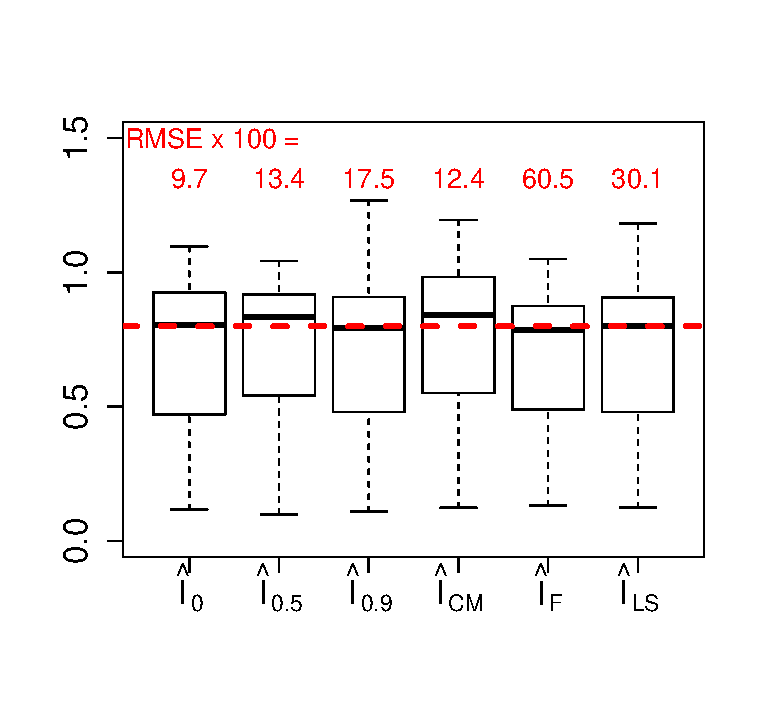
\includegraphics[scale = 0.6, clip = true, trim = 0 0.5in 0 0.5in]{../info_theory_sims/fig1.pdf}
\end{center}
Na\"{i}ve estimator performs best!  $\hat{I}_{LS}$ not effective.
\end{frame}

\begin{frame}
\frametitle{References}
\begin{itemize}
\item Cover and Thomas.  Elements of information theory.
\item Muirhead.  Aspects of multivariate statistical theory.
\item van der Vaart.  Asymptotic statistics.
\end{itemize}
\end{frame}

\end{document}




\begin{itemize}
\item 
\item Define a distribution $p(\bx)$ supported on $\mathcal{X}$.  \emph{In practice, $p(\bx)$ may be represented as a large image database.}
\item Sample stimuli $\bX^{(1)}, \hdots, \bX^{(K)}$ from $p(x)$. \emph{I.e., draw $K$ images from the image database.}
\item For $i = 1,\hdots, K$, present the subject with stimulus
  $\bX^{(1)}$, record the neural response $\bY^{(i, j)}$.  For each
  stimulus, obtain repeats $j = 1,\hdots, r$.
\end{itemize}








